\begin{frame}
	\frametitle{Μέθοδοι και Χρονοδιάγραμμα Υλοποίησης 2/2}

	\centering
	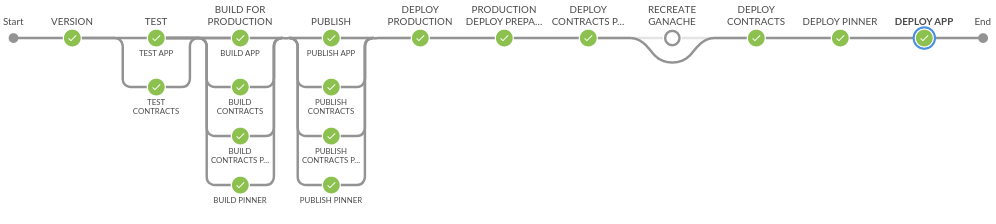
\includegraphics[width=\textwidth]{assets/figures/jenkins-pipeline.png}
\end{frame}

\note{
	Έγινε επίσης δουλειά σε άλλα μέρη της ανάπτυξης όπως το DevOps. Για τις ανάγκες της υλοποίησης, έγινε χρήση του συστήματος CI-CD Jenkins. Το Jenkins είναι ένα αυτοματοποιημένο σύστημα ενσωμάτωσης, ελέγχου και ολοκλήρωσης λογισμικού. Με τη χρήση του CI-CD αυτοματοποιήθηκαν: το χτίσιμο (build) των εφαρμογών μας, ο έλεγχος (testing), η ενσωμάτωση που εδώ αφορά την δημοσίευση του πακεταρισμένου λογισμικού, καθώς και η εγκατάσταση (deployment).
}
